%Notes

% * Exp 1. Precision and recall: detection of inverse transformations

% * Exp 2. Efficiency in special cases

% * Exp 3. Case Studies
%Existing datasets

\section{Experiments}\label{s:exp}
Next, we present experimental results. 

\subsection{Synthetic Data}
In the first set of experiments, we characterize \sys on synthetic data. We generate a dataset with the following schema:
\begin{lstlisting}
City(Name, Abreviation, Population)
\end{lstlisting}
Names are randomly generated from a set of strings scraped from wikipedia, abbreviations are generated from two letters randomly selected from the names, and populations are generated via a Zipfian distribution. This dataset considers multiplicities where there are duplicate (non-erroneous) records.

We consider a number of different anomaly detection criteria:
\begin{itemize}
    \item \textbf{Q1: } All records that violate a one-to-one mapping constraint between \texttt{Name} and \texttt{Abbrevation}. This is a standard functional dependency constraint to detect anomalies~\cite{DBLP:conf/sigmod/ChalamallaIOP14}.
    \item \textbf{Q2: } All records with a population greater than 6 median absolute deviations from the median population. This is a standard quantitative outlier detection condition to detect anomalies~\cite{bailis2016macrobase,scorpion}. 
    \item \textbf{Q3: } All records whose abbreviation has a string length not equal to two. This is a more complex UDF that cannot be addressed by existing work.
\end{itemize}
For each of these anomaly detection criteria, we generate errors in the dataset. For Q1, we select a random subset of each of the records with a particular name and perturb the \texttt{Abbrevation} attribute. For Q2, we randomly generate populations with a population of 0 or one that is much higher than typical and replace a subset of records that satisfy a equality predicate on either \texttt{Name} and \texttt{Abbrevation} or both.
For Q3, we randomly add characters to some records abbrevations.

We consider different parametrized languages for transformations:
\begin{itemize}
    \item \textbf{D1: } All deletions with a single attribute equality predicate.

    \item \textbf{D: } All deletions with a multiple attribute equality predicate. This setting of \sys is the most similar to prior outlier explanation work.

    \item \textbf{R1: } All single attribute find and replace operations.

    \item \textbf{R: } All multiple attribute find and replace operations. This setting of \sys is most similar to prior data cleaning work.

    \item \textbf{M: } All transformations on the population attribute that clip all values above or below a discretized threshold.
\end{itemize}

\subsubsection{Absolute Runtime and Accuracy}
Due to the way that we generated errors, we have a natural notion of ground truth. We know the predicates and transformations used the generate errors, and we can calculate the precision and recall. For a generated dataset of 10000 records, we tuned the error generation process such that approximately 5\% of records are corrupted. The tables (Table \ref{t1} and Table \ref{t2}) show the F1 score of \sys for all combinations of languages and detectors and the runtimes for each of the modes in seconds. We indicate modes for further comparison with existing work. 

\sys provides flexibility to the user the change the language and the quality functions to elict different behaviors. For example, the R and R1 languages are not suited for numerical manipulation. The M language can be used to improve accuracy. The runtime of \sys largely depends on how large the support of the language is. More carefuly designed languages lead to faster and more accurate transformation programs. More complex quality functions only impact runtime in terms of how expensive they are to compute.

\begin{table}[t]
\centering
\caption{The F1 score of \sys for all languages and detector combinations. The starred entries are settings of \sys where there is a plausible comparision with another existing system.}
\label{t1}
\begin{tabular}{
>{\columncolor[HTML]{000000}}l llll}
{\color[HTML]{FFFFFF} }   & \cellcolor[HTML]{000000}{\color[HTML]{FFFFFF} Q1} & \cellcolor[HTML]{000000}{\color[HTML]{FFFFFF} Q2} & \cellcolor[HTML]{000000}{\color[HTML]{FFFFFF} Q3} & \cellcolor[HTML]{000000}{\color[HTML]{FFFFFF} Q123} \\
{\color[HTML]{FFFFFF} D1} & 1.0                                               & 0.89                                              & 1.0                                               & .88                                                 \\
{\color[HTML]{FFFFFF} D}  & 0.84                                              & .86*                                              & 1.0                                               & .79                                                 \\
{\color[HTML]{FFFFFF} R1} & 1.0*                                              & {\color[HTML]{000000} .71}                        & 1.0                                               & .86                                                 \\
{\color[HTML]{FFFFFF} R}  & 0.83                                              & .68                                               & 1.0                                               & .77                                                 \\
{\color[HTML]{FFFFFF} M}  & -                                                 & 1.0                                               & -                                                 & -                                                  
\end{tabular}
\end{table}


\begin{table}[t]
\centering
\caption{The runtime of \sys for all languages and detector combinations. The starred entries are settings of \sys where there is a plausible comparision with another existing system.}
\label{t2}
\begin{tabular}{
>{\columncolor[HTML]{000000}}l llll}
{\color[HTML]{FFFFFF} }   & \cellcolor[HTML]{000000}{\color[HTML]{FFFFFF} Q1} & \cellcolor[HTML]{000000}{\color[HTML]{FFFFFF} Q2} & \cellcolor[HTML]{000000}{\color[HTML]{FFFFFF} Q3} & \cellcolor[HTML]{000000}{\color[HTML]{FFFFFF} Q123} \\
{\color[HTML]{FFFFFF} D1} & 8.1                                               & 3.5                                               & 5.4                                               & 12.9                                                \\
{\color[HTML]{FFFFFF} D}  & 32.9                                              & 24.1*                                              & 21.9                                              & 59.3                                                \\
{\color[HTML]{FFFFFF} R1} & 17.5                                              & {\color[HTML]{000000} 16.5}                       & 17.8                                              & 25.7                                                \\
{\color[HTML]{FFFFFF} R}  & 107.8*                                             & 59.4                                              & 69.3                                              & 136.9                                               \\
{\color[HTML]{FFFFFF} M}  & -                                                 & 0.17                                              & -                                                 & -                                                  
\end{tabular}
\end{table}

\begin{figure*}
    \centering
    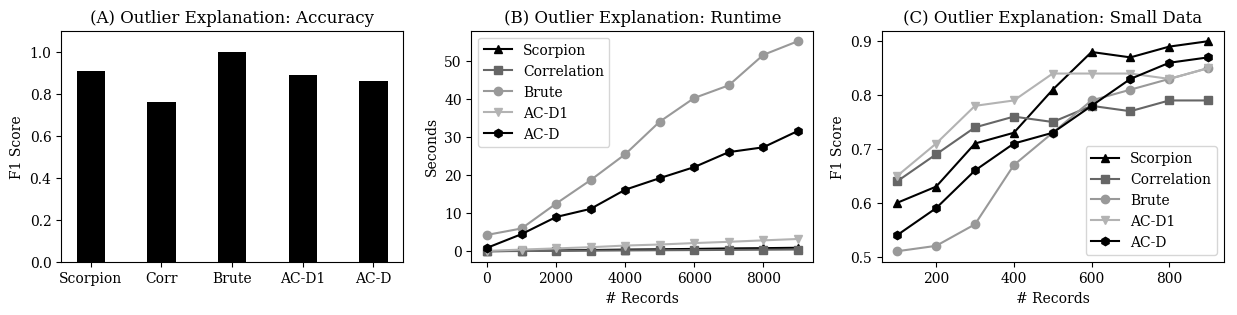
\includegraphics[width=0.8\textwidth]{exp/exp1-new.png}
    \caption{\small Comparison with outlier explanation systems. \label{exp1-new}}
\end{figure*}

\begin{figure*}
    \centering
    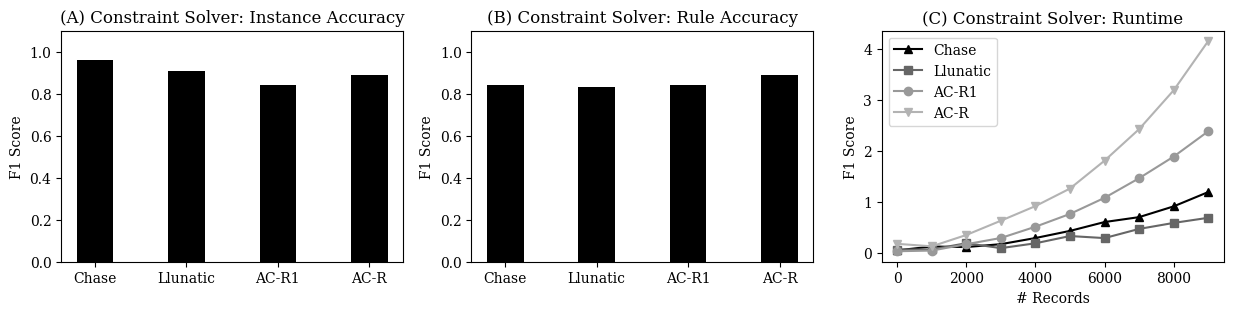
\includegraphics[width=0.8\textwidth]{exp/exp2-new.png}
    \caption{\small Comparison with FD repair systems. \label{exp2-new}}
\end{figure*}

\subsubsection{Comparison to Specialized Systems}
Next, we compare \sys to specialized systems where applicable.  First, we compare \sys to outlier explanation algorithms when the quality function is Q2 (numerical outliers) and the language is only deletions (D1, D). We consider the following alternatives: Scorpion~\cite{scorpion} using a decision tree to extract the predicate, correlation that identifies predicates most correlated with the outliers inspired by and avoids evaluating all subsets of attributes~\cite{bailis2016macrobase}, brute force which enumerates all predicates and returns the one with the highest correlation, \sys with a single attribute predicate (AC-D), and \sys with a multiple attribute predicate (AC). Figure \ref{exp1-new} plots the results for F1 score on 10000 records, runtime, and the F1 score as a function of number of records.
\sys is competitive in terms of accuracy in the specialized cases, but is more expensive in terms of runtime.
The run time of \sys can be improved by changing the language specification (e.g., restricting the search to a single attribute deletion).

Another intriguing result is the accuracy on a small dataset.
Since the alternatives, Scorpion and Brute Force, search over multiple attributes by default. They are susceptible to overfitting to spurious trends when the dataset is small.
\sys with a single attribute predicate actually achieves an improved accuracy result for a smaller dataset.
The flexibility in language can be used as a form of regularization to avoid overfitting.

Next, there is overlap between \sys and data cleaning systems. We next compare to standard functional dependency enforcement algorithms on the quality function Q1 (one-to-one relationship) and the replacement langugages (R1 and R). We compare \sys to a restricted chase algorithm~\cite{benedikt2017benchmarking} and a tuple-generating dependency-based cleaning system called Llunatic~\cite{DBLP:conf/sigmod/DallachiesaEEEIOT13}. The challenge is that these systems do not return rules but return cleaned instances of the database. So, we extract rules from the edits using a decision tree as in scorpion. Then, we compare the systems on two different accuracy metrics: instance accuracy (how well do the transformations recover the true values), and rule accuracy (can we explain the edits with rules). 

Figure \ref{exp2-new} illustrates the results. While \sys is slower than the specialized constraint enforcement systems in terms of runtime, it is competitive in terms of accuracy--especially when it comes to extracting transformation rules. The constraint solving systems operate at a tuple-by-tuple basis and do not necessarily ground their solutions in predicates.

\subsection{Real Case Studies}
Beyond the characterization, we consider 7 case studies applying \sys to real problems. When relevant, we present ``best effort'' comparisons with existing systems--as in the synthetic experiments.

\stitle{Flight} The flight dataset~\cite{data-flights} contains arrival time, departure time, and gate information aggregated from 3 airline websites (AA, UA, Continental), 8 airport websites (e.g., SFO, DEN), and 27 third-party websites.
There are 1200 flight departures and arrivals at airline hubs recorded from each source.  Each flight has a unique and globally consistent ID, and the task is to reconcile data from different sources using the functional dependency \texttt{ID$\rightarrow$ arrival, departure, gate information}.


\stitle{FEC} The election contributions dataset has 6,410,678 records, and 18 numerical, discrete, and text attributes. This dataset records the contribution amount and contributor demographic information e.g., name, address, and occupation.  The task is to enforce \texttt{city$\rightarrow$zipcode}, and match occupation to a codebook on canonical occupations.  The quality function is 1 if the occupation is in the codebook, and 0 otherwise; we penalize the edit distance between the original and edited occupation values.

\stitle{Malasakit} This dataset contains 1493 survey disaster preparedness responses from the Philippines, with 15 numeric and discrete attributes. The task removes improper numerical values and remove dummy test records. This consists of domain integrity constraints that force the values to be within a certain dictionary.

\stitle{Physician} This dataset from Medicare.gov contains 37k US physican records, 10 attributes, with spelling errors in city names, zipcodes, and other text attributes. We use the rules described in~\cite{rekatsinas2017holoclean}, which consists of 9 functional dependencies for error detection. 

\stitle{Census} This US adult census data contains 32k records, and 15 numeric and discrete attributes.  There are many missing values coded as 999999.  The task is to clean numeric values to build a classification model that predicts whether an adult earns more than $\$50k$ annually. 

\stitle{EEG}  The 2406 records are each a variable-length time-series of EEG readings (16 numeric attributes), and labeled as ``Preictal'' for pre-seizure and ``Interictal'' for non-seizure.  The goal is to predict seizures based on 32 features computed as the mean and avriance of the numeric EEG attributes.  The task is to identify and remove outlier reading values.  

\stitle{Terrorism} The Global Terrorism Database~\cite{data-terrorism} is a dataset of around terrorist attacks scraped from news sources.  Each record contains the date, location, details about the attack, and the number of fatalities and injuries.  The dataset contains a mixture of data errors:
(1) there are many duplicates for the same terrorist incident,
(2) many missing values in the fatalities and injuries attributes are encoded as zeros, which overlaps with attacks that did not have any fatalities/injuries, and
(3) the location attributes are inconsistently encoded.  
We used the dataset from 1970, and there are $170000$ records.  
We downloaded this dataset and sought to understand whether terrorist attacks have become more lethal than they were in the 1970s.  To do so, we hand cleaned the records to create a gold standard.  It turns out that, in this dataset, attacks have become more lethal, but fewer in number than 50 years ago.  This task was intentionally open-ended to represent the nature of the iterative analysis process.


\begin{figure}
    \centering
    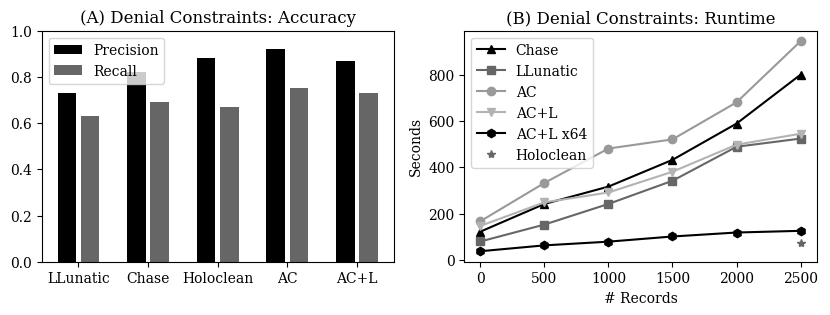
\includegraphics[width=\columnwidth]{exp/exp1.png}
    \caption{\small Comparison with denial constraint systems on the Flight dataset.  (A) \sys (AC) matches or exceeds the accuracy of the specialized systems.  (B) The structure of the data errors, along the learning and parallelization (AC+L x64) lets \sys scale sub-linearly and outperform all but HoloClean's reported runtimes.  \label{exp1a}}
\end{figure}

\subsection{Constraint Violations}
Denial constraints express a wide range of integrity constraints and form the basis of many data cleaning systems.  We can compose a quality function that quantifies the number of constraint violations and find transformations that reduce the number of violations. For \sys, we search over single attribute find and replace transformations (R1 in the synthetic experiments). We quantify the precision and recall of the transformations discovered. We use the Flight dataset for these experiments. 

\stitle{Baselines} We run against (1) Llunatic, a denial constraint-based cleaning system~\cite{DBLP:conf/sigmod/DallachiesaEEEIOT13} implemented in C++ on top of PostgreSQL\footnote{Constraints are specified as Tuple-Generating Dependencies}, and (2) a restricted chase algorithm~\cite{benedikt2017benchmarking} implemented in Python. We compare against the chase because a large portion of denial constraints are functional dependencies, and can be resolved using fixed-point iteration.  We report numbers from the recent Holoclean publication~\cite{rekatsinas2017holoclean} that used the same datasets and constraints, but did not run the experiment ourselves.

\stitle{Results} Figure \ref{exp1a}a shows the precision and recall of each approaches based on known ground truth. \sys matches or beats the accuracy of the baselines, however its runtime (AC) without any learning scales poorly compared to alternatives (Figure~ \ref{exp1a}b).  Using learning (AC+L) shows performance on par with LLunatic, and parallelization on 64 threads is comparable to Holoclean's reported runtime. The results suggest that learning exhibits sublinear scaling due to \sys learning more effective pruning rules as it sees more data.  These performance gains are at the expense of slightly reduced accuracy. 

We also evaluated \sys (single threaded, without learning) on the FEC, Malasakit, and Physician datasets.  Their precision, recall, and runtimes are as follows: 
FEC: $94\%$ prec, $68\%$ rec, $5$hrs; 
Malasakit: $100\%$ prec, $85\%$ rec, $0.39$hrs;
Physician: $100\%$ prec, $84\%$, $3.4$hrs.


\begin{figure}
    \centering
    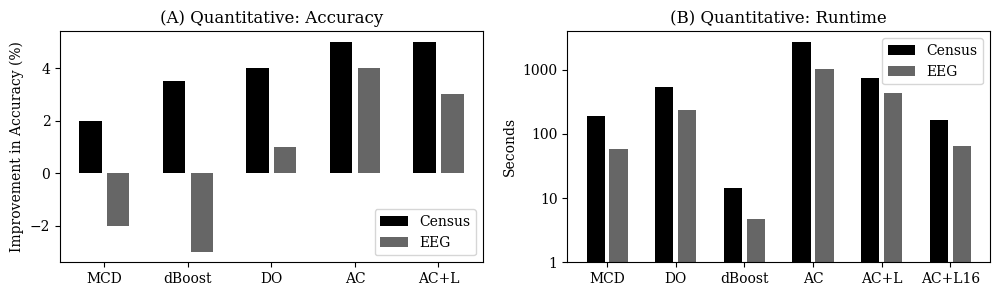
\includegraphics[width=\columnwidth]{exp/exp2.png}
    \caption{\small Numerical Transformations on census and EEG datasets for a classification application.  \sys tranformation can clip outliers or set them to a default value. (A) \sys has a higher accuracy than outlier detection algorithms (MCD, dBoost), and \sys with a single transform template (DO).  (B) Optimizations improve \sys runtime by over an order of magnitude.  \label{exp2a}}
\end{figure}

\subsection{Numerical Transformations}\label{s:expquant}
This experiment performs numerical transformations on machine learning data.  We explore to what extent the transformations provided by \sys can be used to improve the performance of a downstream data product such as machine learning. In these applications, prediction labels and test records are typically clean and available (e.g., results of a sales lead), whereas the training features are often integrated from disparate sources and exhibit considerable noise (e.g., outliers).  Our quality function is simply defined as the model's accuracy on a training hold-out set, and we report the test accuracy on a separate test set.

We trained a binary classification random forest model using \texttt{sklearn} on the Census and EEG datasets.  We used standard featurizers (hot-one encoding for categorical data, bag-of-words for string data, numerical data as is) similar to~\cite{gokhale2014corleone}. 
We split the dataset into 20\% test and 80\% training, and further split training into 20/80 into hold-out and training.  We run the search over the training data, and evaluate the quality function using the hold-out.  Final numbers are reported using the test data.

We defined the following three data transformation templates that sets numerical attribute values in $R$ if they satsify a predicate:

{\small
\begin{itemize}[leftmargin=*, topsep=0mm, itemsep=0mm]
  \item \stitle{\textsf{clip\_gt(attr, thresh)}} $R.attr = thresh$ if $R.attr>thresh$
  \item \stitle{\textsf{clip\_lt(attr, thresh)}} $R.attr = thresh$ if $R.attr<thresh$
  \item \stitle{\textsf{default(attr, badval)}} $R.attr$ set to mean val if $R.attr=badval$
\end{itemize}
}

\stitle{Baselines} We compare with 4 baselines: {\it No Transformation (NC)}, {\it Minimum Covariance Determinant (MCD)} is a robust outlier detection algorithm used in~\cite{bailis2016macrobase} and sets all detected outliers to the mean value, {\it dBoost} uses a fast partitioned histogram technique to detect outliers~\cite{mariet2016outlier}, and {\it Default Only (DO)} runs \sys with only the \textsf{default()} transformation.  

\stitle{Results} The classifer achieves 82\% and 79\% accuracy on the uncleaned census and EEG data, respectively.  Most outliers in the census data are far from the mean, so MCD and dBoost can effectively find.  Further, setting census outliers to the mean is sensible. However, the same fix is not appropriate for the EEG data; it is better to clip the outlier values, thus MCD, dBoost, and DO have negligible or negative impact on accuracy.  When we realized this from running DO, it was straightforward to add the clipping transformations to the language, and with no other changes, re-run \sys with drastically improved EEG accuracies.  

Vanilla \sys (AC) is nearly $10\times$ slower than MCD, but the adding learning and 16-thread parallelization  matches MCD's runtimes.  dBoost is specialized for fast outlier detection and \sys is unlikely to match its runtime.  


\begin{figure}[ht]
    \centering
    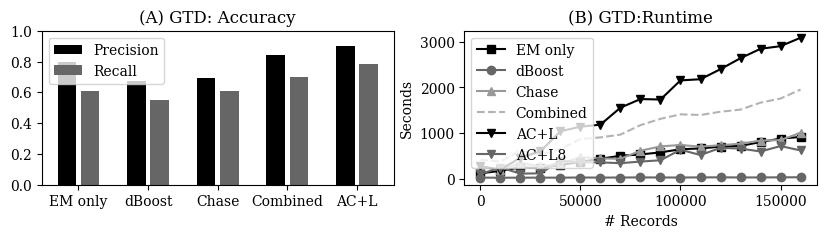
\includegraphics[width=\columnwidth]{exp/exp7.png}
    \caption{The Global Terrorism Database is a dataset of terrorist attacks scraped from news sources since 1970. (A) Shows that \sys can integrate many different forms of transformations that were previously handled by disparate systems, (B) \sys achieves a competitive runtime to using all of the different system and accounting for data transfer time between them. \label{exp7a}}
\end{figure}

\subsection{Mixing Error Classes}\label{s:expterror}
This experiment, we use the multi-error Terrorism dataset~\cite{data-terrorism}. 

\stitle{Baselines} We hand-coded blocking-based entity matching (EM)  and restricted chase (FD) algorithms in Python, and used dBoost for missing values.  We also ran EM, dBoost, and Chase serially on the dataset (Combined). We use that combination to generate transformation explanations.

%algorithm that uses blocking to handle duplicate records.  We modeled the missing values as an outlier cleaning problem and used the dBoost~\cite{} library (dBoost). We modeled the location inconsistencies as a functional dependency problem and implemented a restricted chase algorithm (Chase).  


\stitle{Results} \Cref{exp7a}a shows that combining  all three classes of errors within the same \sys framework (AC) achieves higher precision and recall than all baselines.  In fact, the combined baselines still does not achieve \sys's level of accuracy because the  operations need to be interleaved differently for different blocks.   Although \sys is slower than any individual baseline, parallelizing \sys to 8 threads is faster than the combined baseline by 2x. 


% Error type (1) is best handled with a blocking and matching entity matching approach. Error type (2) is best handled with an outlier detector, where outliers are replaced with null values. Error type (3) is best addressed by a Functional Dependency.
% Figure \ref{exp7a}a shows how each individual system is not sufficient to clean the data.
% For (1) and (3), we coded a specialized algorithm in Python to address those errors.
% For (2), we used the dBoost library.
% \sys can model all of these in a single framework and can get the best combined performance.
% \sys achieves the highest precision and recall.
% \sys also achieves a competitive runtime to using all of the different system and accounting for data transfer time between them.

 \begin{figure*}[t]
\centering
 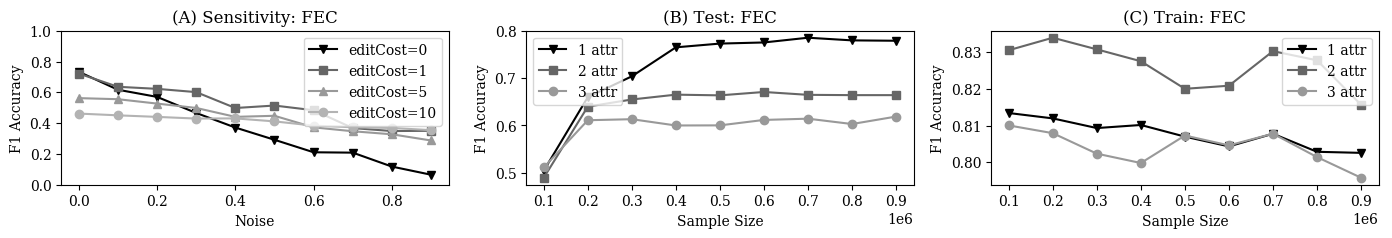
\includegraphics[width=\textwidth]{exp/exp5.png}
 \caption{\small (A) Regularization by increasing an editCost penalty makes \sys more robust to noisy (mis-specified) quality functions, (B-C) overly expressive transformation templates can lead to overfitting (2 attr) or an infeasibly large search space (3 attr).  
 \label{fig:sensitivity}}
\end{figure*}

 \begin{figure*}[t]
\centering
 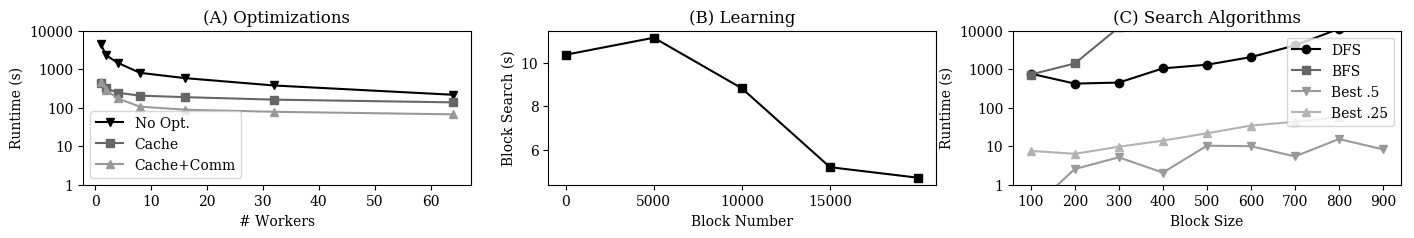
\includegraphics[width=\textwidth]{exp/exp6.png}
 \caption{\small 
   (A) Both the materialization (Cache) and distributed communication (Comm) optimizations contribute to improved scale-out runtimes.
   (B) The learned pruning rules improve the search costs for each subsequent block-wise partition.  
   (C) Best-first search is better than BFS and DFS; reducing $\gamma$ prunes more candidates at the expense of lower accuracy.  
 \label{fig:opt}}
\end{figure*}


\subsection{\sys In Depth}
This subsection uses the FEC setup to study the parameters that affect \sys's accuracy and runtime, the robustness of its transformation programs, and its algorithmic properties.

\subsubsection{Algorithmic Sensitivity}

\stitle{Partitioning} Partitioning the dataset into smaller blocks effectively reduces the problem complexity.  This can have tremendous performance benefits when each block exhibits very few errors that are independent of the other blocks.  \Cref{fig:microbenchmarks}a shows the performance benefits when varying the block size; we define the blocks by partitioning on three different attributes that have different domain sizes.  Reducing the block size directly improves the runtime; the search is effectively non-terminating when blocking is not used.    

\stitle{Language} \Cref{fig:microbenchmarks}b fixes the input to a single block, and evaluates the runtime based on the size of the language $|\Sigma|$.  Increasing the transformations increases the branching factor of the search problem. The search time is exponential in the language, however \sys's learning optimization can identify a pruning model that reduces the runtime to linear.

\stitle{Coupling in the Quality Function} The complexity of the quality function directly affects search time.  A cell-separable quality function is the simplest to optimize because each cell in the relation can be analyzed and cleaned in isolation.  In contrast, a quality function that couples multiple records together is more challenging to optimize because a longer sequence of transformation may be needed to sufficiently clean the records and improve the quality function.  

We evaluate this by artificially coupling between 1-10 records together, and creating a quality function that only improves when an attribute of the coupled records all have the same value.  We perform this coupling in two ways: {\it Random} couples randomly selected records, whereas {\it Correlated} first sorts the relation an attribute and couple records within a continuous range.  We expect that the random coupling requires individual operations for each record based on their IDs, whereas the correlated setting both allows \sys to exploit the correlated structure to learn effective pruning rules and to clean the coupled records using a single operation.  \Cref{fig:microbenchmarks}c shows that this is indeed the case when running \sys on a single fixed-size block. {\it Random} slows down exponentially with increased coupling, whereas {\it Correlated} increases linearly.

% The nature of the quality function also affects the search time. Quality functions that couple multiple records together are harder to optimize (Figure \ref{fig:microbenchmarks}c).
% Consider a function that requires that two different records must have the same attribute values.
% More transformations have to be achieved in a particular sequence before an improvement in quality is observed. 
% We selected between 1-10 records at random in each block and created a quality function that coupled these records together.
% As the degree of coupling increases, the search time grows quite drastically.
% We repeated the same experiment where now coupling is correlated with the data, i.e., we sort one of the attributes and couple ``nearby'' records.
% \sys performs significantly better on this version of the task.
% This is due to the learned pruning in \sys.
% Sorting the attributes introduces a systematic correlation in the quality function.
% \sys quickly learns a model which learns this correlation and uses that to prune the search space.

\stitle{Quality Function Complexity} Finally, we incrementally increase the quality function's complexity and show haw it affects the accuracy.  We add the following constraints in sequence: one functional dependency (FD), a second FD, an entity resolution similarity rule, and a third FD.  We define the quality function as the sum of each constraint's quality function.   \Cref{fig:microbenchmarks}d shows that the F1 accuracy decreases as more constraints are added, however the F1 score is still above $75\%$.  




\subsubsection{Generalization and Overfitting}\label{s:expoverfit}
An important characteristic of generating transformation solutions as {\it programs} is that we can evaluate the program's robustness in terms of machine learning concepts such as overfitting and generalization.    To this end, we examine two concepts in the context of data transformations: regularizaton and overfitting.  We also find that \sys's high level interface is helpful for iteratively tuning the transformation process.

\stitle{Regularization}  Misspecified quality functions can cause \sys to output poorly performing transformation programs.  We simulate this by adding random noise to the output of the quality function. \Cref{fig:sensitivity}A plots the F1-score of \sys on the FEC experiment while varying the amount of noise.  As expected, the output program's F1-score rapidly degrades as the noise increases.  

Machine learning uses regularizing penalty terms to prevent overfitting.  We can similarly add a penalty to the quality function to prevent too many edits.  Each line line shows the edit cost penalty and shows that although the F1 is lower when there is no noise, \sys is more robust to larger amounts of noise. 

\stitle{Overfitting} In machine learning, over-parameterized models may be susceptible to overfitting.  A similar property is possible if the language $\Sigma$ is overly expressive.  We use a transformation template that finds records matching a parameterized predicate and sets an attribute to another value in its instance domain.   We then vary the language expressiveness by increasing number of attributes in the predicate between 1 and 3.  Finally, we run \sys on a training sample of the dataset (x-axis), and report F1 accuracy on the training and a separate test sample (\Cref{fig:sensitivity}B-C).  Note that overfitting occurs when the training accuracy is significantly higher than test accuracy.

Indeed we find an interesting trade-off.  The 1 attribute predicate performed worst on the training sample but outperformed the alternatives on the test sample.  The 2 attribute predicate was more expressive and overfit to the training data.  Finally, the 3 attribute predicate is overly expressive and computationally difficult to search.  Thus, it did not sufficiently explore the search space to reliably identify high quality transformation programs. 

\stitle{Discussion} We have shown that data transformations can overfit, and believe this is a potential issue in {\it any} transformation procedure. These results highlight the importance of domain experts to judge and constrain the problem in ways that will likely generalize to future data. Further, it shows the value of a high-level interface that experts can use to express these contraints by iteratively tuning the quality function and transformation language. 

% and evaluate the training and test        Figure \ref{fig:sensitivity}B-C illustrates another interesting aspect of \sys, namely, a property akin to overfitting in machine learning.
% We parametrized the transformation language with single attribute, double attribute, and triple attribute predicates.
% Then, we applied \sys to sample of data.
% We measured the ``in-sample error'' Figure \ref{fig:sensitivity}C, which is the F1 score with records inside the sample, and the ``out-of-sample'' error which is the F1 score on unseen records.
% The more expressive two attribute predicates are most accurate on the in-sample metric, however, we not as accurate as the single attribute predicates on the out-of-sample metric.
% The three sample predicates were very computationally expensive to search so the results are less reliable.
% This result highlights an important point overly specific rules may not apply to future data, and overly general rules, might introduce unwanted side-effects.


\subsubsection{Scaling}
Next, we present preliminary results illustrating the scaling properties of \sys. 

\vspace{1em}

\stitle{Parallelization Optimizations} The experiments run on a cluster of 4 mx.large EC2 instances, and we treat each worker in a distributed (not shared-memory) fashion.   \Cref{fig:opt}a shows the benefits of the materialization and communication optimizations in \Cref{s:parallel}.  {\it No opt.} simply runs best-first search in parallel without any materialization; workers only synchronize at the end of an iteration by sending their top-$\gamma$ candidate programs to the driver, which prunes and redistributes the candidates in the next iteration.  {\it Cache} extends No opt by locally materializing parent programs, and {\it Cache+Comm} further adds the communication optimizations for distributed parallelization.   

The single threaded No Opt setting runs in $4432$s, and the materialization optimization reduces the runtime by $10\times$ to $432$s.   Scaling out improves all methods: at 64 workers, {\it Cache+Comm} takes 67s while {\it Cache} takes 137s.  Surprisingly, although {\it No Opt} with 64 workers is slower than {\it Cache+Comm} by $10\times$, it scales the best because it only synchronizes at the end of an iteration and only communicates candidate programs and their quality values.  In contrast, the alternative methods may communicate materialized relation instances.  

\stitle{Within-Block Learning} Although we have shown how learning reduce the overall search runtime, we show that learning also improves the search speed for individual blocks.  We run single-threaded \sys and report the time to evaluate each block.  \Cref{fig:opt}b shows the $i^{th}$ block that is processed on the x-axis, and the time to process it on the y-axis.   We see that as more blocks are cleaned, the learned pruning classifier is more effective at pruning implausible candidate programs.  This reduces the per-block search time by up to $75\%$.  

\stitle{Search Algorithm Choice} \Cref{fig:opt}c shows that best-first search out-performs naive depth and breadth first search.  We also report \sys when $\gamma=\{0.5, 0.25\}$.  We see that as the block size increases, DFS and BFS quickly become infeasible, whereas \sys runs orders of magnitude more quickly.  In addition, reducing $\gamma$ improves the runtime, however can come at the cost of reduced accuracy by pruning locally sub-optimal but globally optimal candidate programs.  



\subsubsection{Program Structure}
Finally, we present results describing the structure of the data transformation programs found with \sys.
It is often the case that the program found by \sys is a concise description of the needed data transformation operations, that is, the total number of cell edits is much larger than the length of the program.
We consider the FEC dataset, the EEG dataset, and GTD dataset.

Sometimes, the program (FEC and GTD) encodes a significant amount of literal values. This happens in entity matching type problems. For these problems, the program length is relatively large, however, the number of cells modified is even larger (up to 10x more).
For datasets like the EEG dataset, the program is very concise (26x smaller than the number of cells modified).
Numerical thresholds are generalize better than categorical find-and-replace operations.

\begin{table}[ht!]
\centering
\label{my-label}
\begin{tabular}{|l|l|l|}
\hline
    & Program Length & Cells Modified \\ \hline \hline
FEC & 6416           & 78342          \\ \hline
EEG & 6              & 161            \\ \hline
GTD & 1014           & 104992 \\ \hline
\end{tabular}
\end{table}
